\documentclass[lettersize,journal]{IEEEtran}
\usepackage{amsmath,amsfonts}
\usepackage{algorithmic}
\usepackage{array}
\usepackage[caption=false,font=normalsize,labelfont=sf,textfont=sf]{subfig}
\usepackage{textcomp}
\usepackage{stfloats}
\usepackage{url}
\usepackage{verbatim}
\usepackage{graphicx}
\usepackage{cite}
\usepackage{multirow}
\hyphenation{op-tical net-works semi-conduc-tor IEEE-Xplore}
\def\BibTeX{{\rm B\kern-.05em{\sc i\kern-.025em b}\kern-.08em
    T\kern-.1667em\lower.7ex\hbox{E}\kern-.125emX}}
\usepackage{balance}
\begin{document}
\title{A Dual Branch Multi-scale Image Dehazing Network Based on High Quality Codebook Priors
\author{Xuehui Yin, Peixin Wu, Zehong Li,~\IEEEmembership{Senior Member,~IEEE}}
\thanks{This work was supported in part by the National Natural Science Foundation of China under Grant 61701060, in part by the Scientific and Technological Research Program of Chongqing Municipal Education Commission under Grant KJQN202000619.
	
Xuehui Yin, Peixin Wu are with the School of Software Engineering, Chongqing University of Posts and Telecommunications, Chongqing 400065, China (e-mail: yinxh@cqupt.edu.cn; w1066365803@163.com). 

Zehong Li is with the State Key Laboratory of Electronic Thin Films and Integrated Devices, University of Electronic Science and Technology of China (UESTC), Chengdu 611731, China, also with Shenzhen Institute for Advanced Study, UESTC, Shenzhen 518110, China, and also with Chongqing Institute of Microelectronics Industry Technology, UESTC, Chongqing 401331, China (e-mail: lizh@uestc.edu.cn).
}}

\markboth{IEEE Transactions on Instrumentation and Measurement}%
{How to Use the IEEEtran \LaTeX \ Templates}

\maketitle

\begin{abstract}
Non-homogeneous haze removal has attracted enormous interest in computer vision owing to its critical impact on image quality degradation and downstream visual tasks. Existing methods often fail to address non-homogeneous haze due to limited prior knowledge and insufficient training data. While deep learning-based approaches have advanced image dehazing, their reliance on homogeneous haze assumptions and handcrafted priors leads to suboptimal performance in complex real-world scenes with spatially varying haze concentrations. The aim of this study is to investigate a codebook-driven dual-branch network for robust prior learning and detail-preserving non-homogeneous haze removal. We established a high-quality codebook to capture clear image textures as dehazing priors, coupled with a pyramid dilated neighborhood attention encoder for multi-scale haze feature extraction and an enhanced decoder with multi-attention mechanisms. A dual-branch architecture was designed to address dense haze regions through feature fusion. These findings open new avenues for image restoration under complex degradation scenarios by integrating generative priors with attention-aware feature learning, potentially benefiting autonomous driving and remote sensing systems.
\end{abstract}

\begin{IEEEkeywords}
Image dehazing, codebook, a two-branch network, multi-scale, neighborhood attention.
\end{IEEEkeywords}


\section{Introduction}
\IEEEPARstart{H}{aze} is an aerosol system composed of numerous tiny water droplets suspended in the near-ground air, serving as one of the primary causes of image blurring, color distortion, and contrast reduction. The hazy image degradation model based on atmospheric light single scattering phenomenon~\cite{mccartney1976optics}~\cite{narasimhan2002vision} can be represented as:

\begin{equation}
	\label{scattering_model}
	I(x) = J(x)t(x) + A(1 - t(x))
\end{equation}

\noindent where $I(x)$ denotes the hazy image, and $J(x)$ is its corresponding ground truth. $A$ is the environment lighting, and the transmission map is represented by $t(x) = e^{\beta d(x)}$ which depends on scene depth $d(x)$ and haze density coefficient $\beta$. 

The outdoor visual systems such as autonomous driving, video surveillance, military reconnaissance, and remote sensing imagery are affected by hazy conditions, leading to a decrease in the accuracy of information acquisition from captured images. As the haze intensity increases and non-homogeneous haze emerges, the image quality deteriorates rapidly, resulting in color distortion, blurred features, reduced contrast, and other visual quality degradations. Consequently, it becomes challenging to identify objects and backgrounds within the image, significantly impacting the effectiveness of subsequent visual tasks such as semantic segmentation and object detection in computer vision. Therefore, it is necessary to preprocess the images to mitigate the impact of dense haze on image quality.

Although existing dehazing methods based on deep learning have made significant progress, image dehazing remains a highly ill-posed problem that often requires prior knowledge to effectively tackle. Earlier dehazing methods, such as~\cite{he2010single, cai2016dehazenet, li2017aod} are largely based on empirical observations and manually set priors, which resulted in limitations when applied to complex or non-homogeneous haze scenarios. These methods often underperform in real-world applications where haze is not uniformly distributed, leading to residual haze in regions with large depth variation~\cite{liu2019griddehazenet, qin2020ffa}. Recently, more advanced techniques have incorporated deep learning strategies, such as~\cite{guo2022image, song2023vision, yu2021two, jin2022structure, liu2023data}, improving performance in handling dense haze and depth variations. However, many of these methods still struggle with preserving fine image details in regions affected by dense haze.

In contrast, our approach introduces a dual-branch multi-scale image dehazing network, leveraging a high-quality codebook~\cite{esser2021taming} to integrate robust prior knowledge for texture and detail preservation. Additionally, we propose a feature pyramid encoding module based on dilated neighborhood attention~\cite{hassani2022dilated} and a multi-scale channel attention mechanism to address the challenge of dehazing in regions with complex haze distributions. Finally, a dual-branch network is utilized to integrate these methods, resulting in our proposed network.

The contributions of our work can be summarized as follows:

\begin{list}{}{}
\item{1) We employ the VQGAN generative model to train a high-quality codebook as a prior, thereby complementing robust prior knowledge and mitigating the impact of haze features in the dehazing network.}

\item{2) We design a feature pyramid encoding module based on dilated neighborhood attention and an enhanced decoding module incorporating pixel-wise and channel-wise attention. By leveraging a dual-branch multi-scale network structure, we improved the feature extraction capability for regions with dense haze in images.}

\item{3) We propose a dual-branch multi-scale image dehazing network that integrates high-quality priors from a codebook. This method preserves texture details and mitigates haze effects. A feature pyramid encoder and multi-scale attention mechanisms enhance feature extraction, leading to superior performance in dense haze regions.}
\end{list}
 
\begin{figure*}[!t]
	\centering
	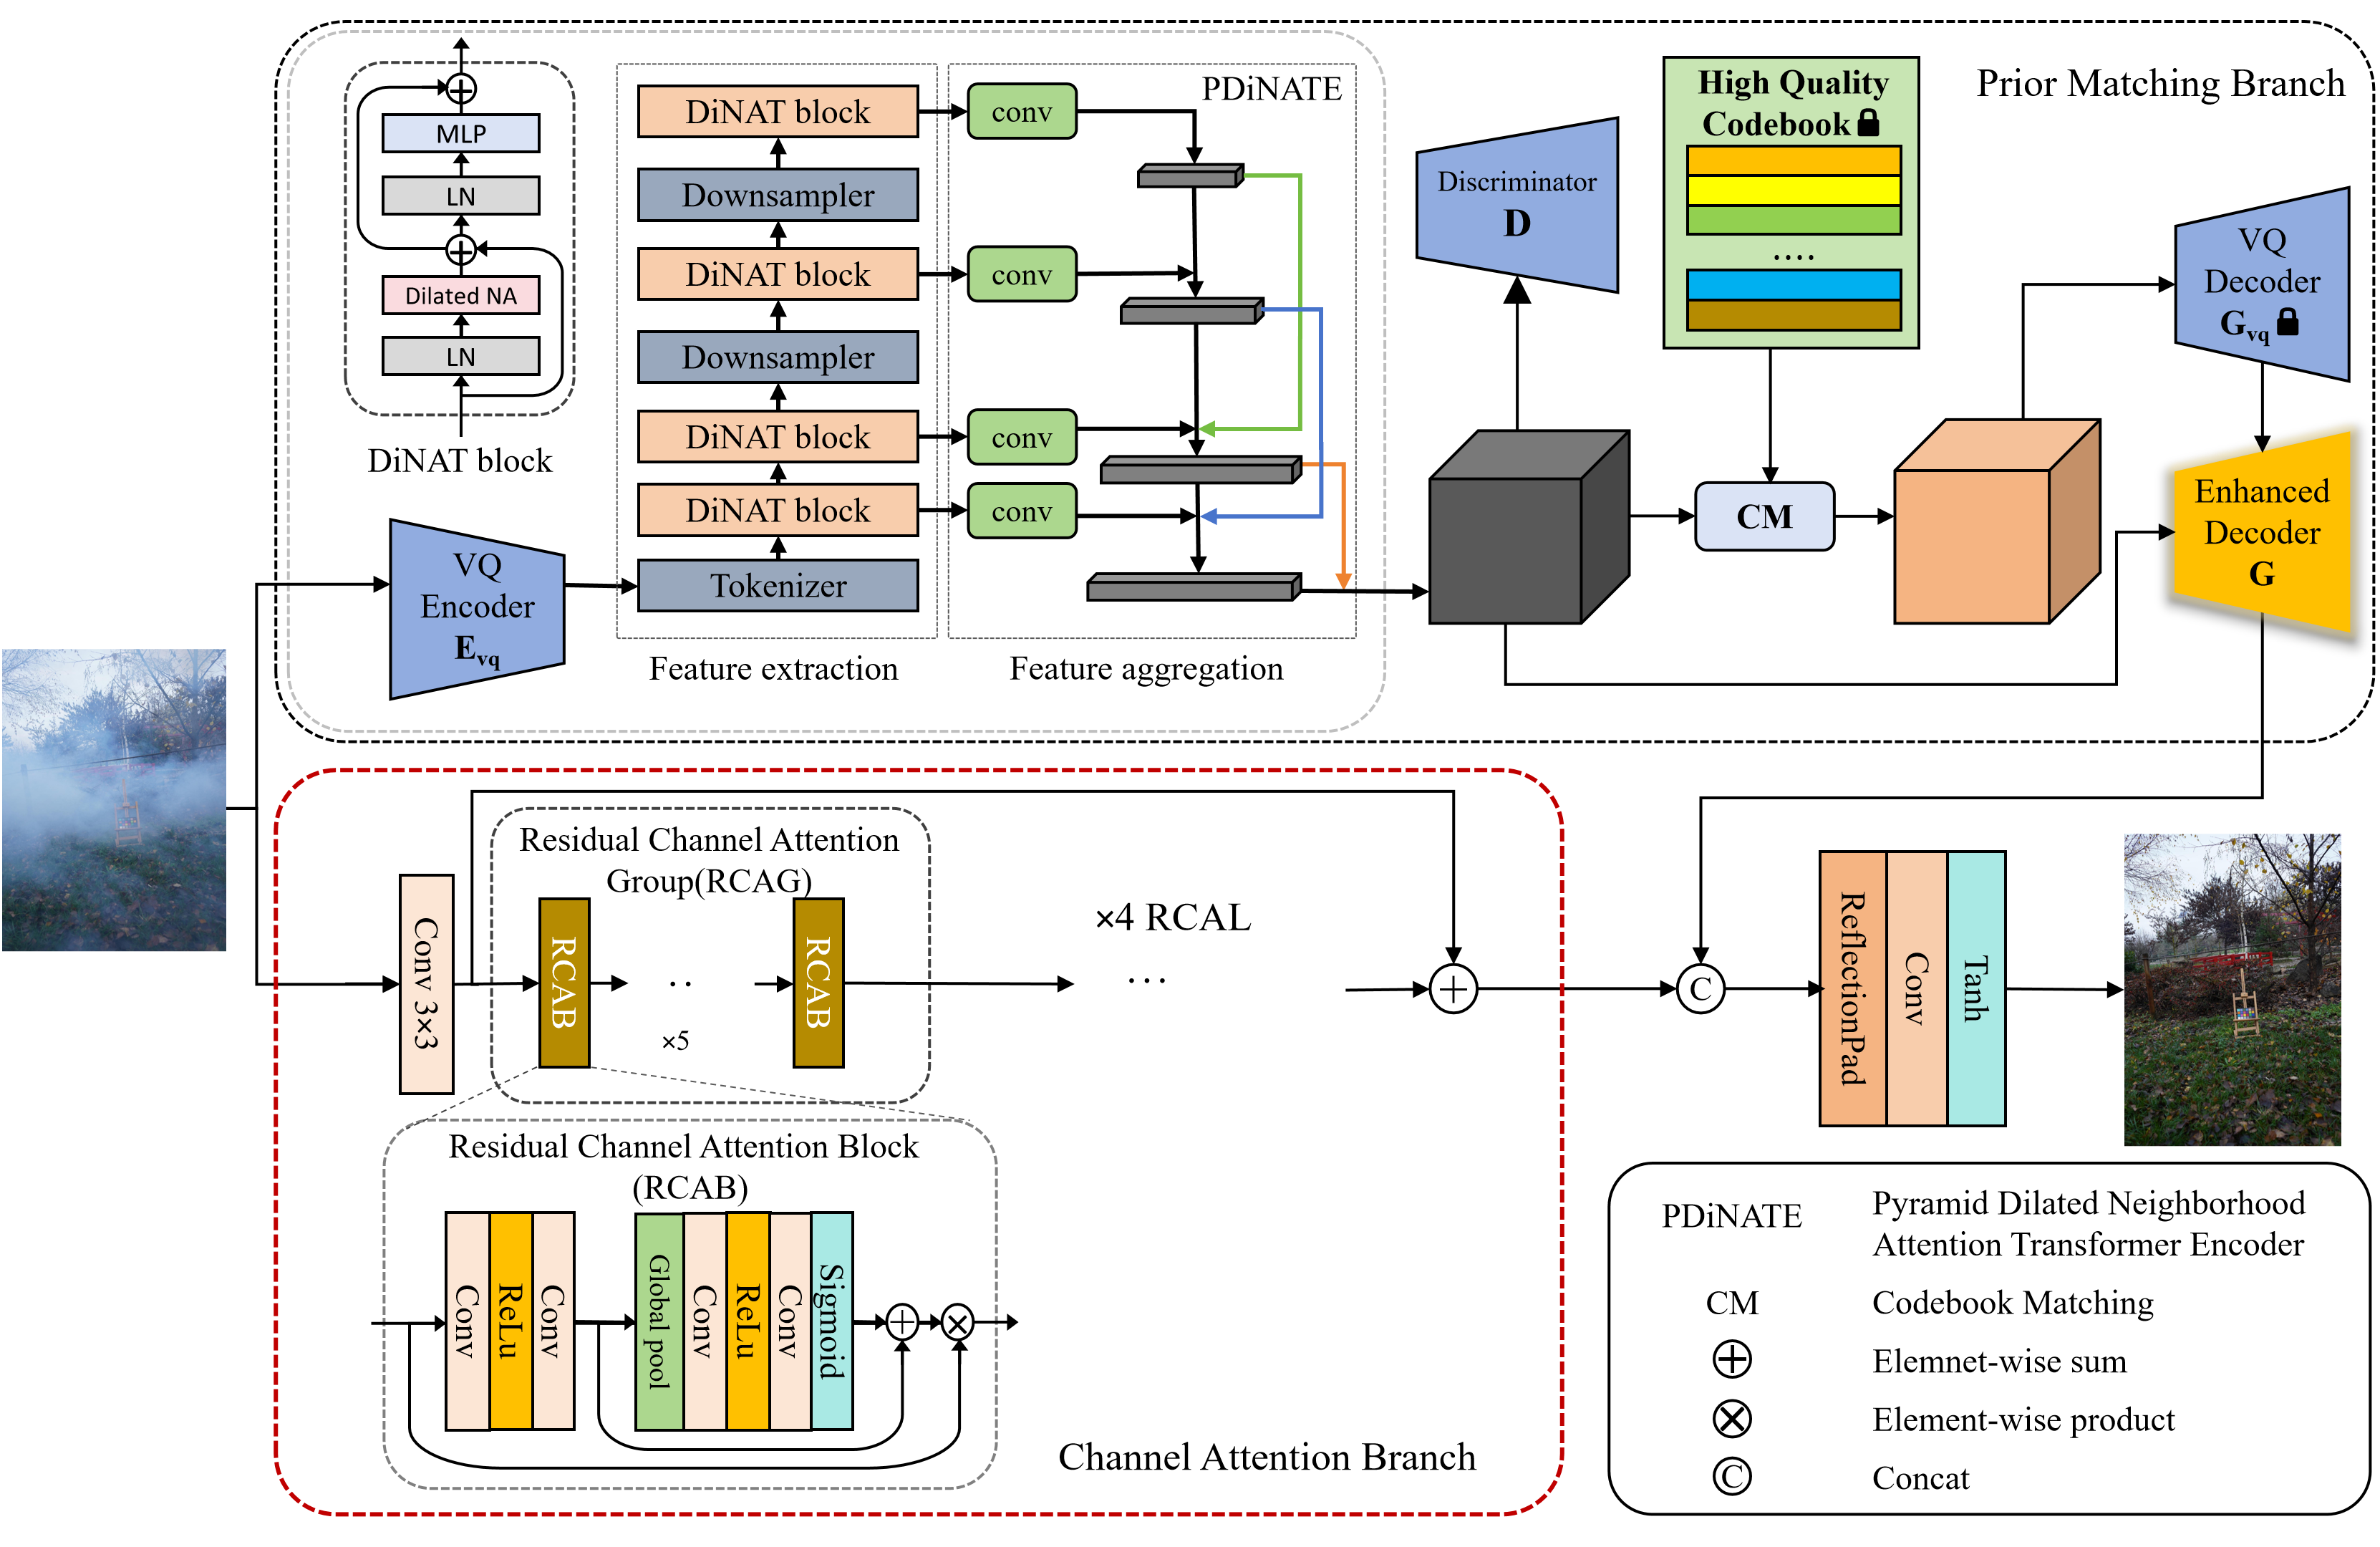
\includegraphics[width=7in]{network_architecture}
	\caption{An overview of our network. This model consists of two branches: prior matching branch and channel attention branch. Hazy image is processed separately by two branches, each outputting a feature map. Then, a feature fusion tail is used to fuse the feature maps of the two branches, and finally generate a hazy-free image.}
	\label{fig0}
\end{figure*}

\section{RELATED WORK}
\subsection{Prior-Based Dehazing Methods}
Early prior-based dehazing methods relied on physical priors. The seminal work by He et al.~\cite{he2010single} pioneered the dark channel prior, which statistically observes that haze-free images contain pixels with near-zero intensity in at least one color channel. Subsequently, Zhu et al.~\cite{zhu2015fast} introduced the color attenuation prior, establishing a linear relationship between haze concentration and scene depth through brightness-saturation discrepancy analysis. This depth information is subsequently employed to recover the haze-free image through atmospheric scattering modeling.

\subsection{Learning-Based Dehazing Methods}
Recent learning-based approaches have advanced feature integration strategies. Liu et al.~\cite{liu2019griddehazenet} introduced a grid network with attention mechanisms for multi-scale processing, effectively combining hierarchical features. Qin et al.~\cite{qin2020ffa} developed an end-to-end network using channel attention to dynamically weight features, eliminating sampling operations while enhancing feature discriminability through residual attention blocks. Yin et al.~\cite{yin2023multiscale} propose a novel multiscale depth information fusion enhancement network to improve dehazing ability in scenes with large depth changes. 

Transformer~\cite{vaswani2017attention} was initially proposed for natural language processing tasks, capturing non-local interactions between words through the stacking of multi-head self-attention mechanisms and feed-forward layers. DeHamer~\cite{guo2022image} combined convolutional neural networks and Transformer for image dehazing, aggregating long-term attention in Transformer and local attention in convolutional neural network features. Dehazeformer~\cite{song2023vision} proposed an offset window partitioning scheme based on reflection padding and cropping, allowing the mask multi-head self-attention to discard part of the mask and achieve a constant window size.

However, there are currently two major challenges in applying Transformer to the image field. First is the large variation in visual entities, and the performance of Transformer may not be well in different scenes. Second is that the image resolution is high and there are many pixels, so the global self attention mechanism in Transformer leads to a large amount of computation.

In recent years, people have made a lot of achievements in heavy haze and non-homogeneous haze. Among them, TNN~\cite{yu2021two} introduced a dual-branch neural network, using Res2Net pre-trained on ImageNet~\cite{deng2009imagenet} and residual channel attention network~\cite{zhang2018image}, and then through a learnable tail to fuse the features of the two branches, committed to solve non-homogeneous haze. FogRemoval~\cite{jin2022structure} combines the structural representation of ViT\cite{dosovitskiy2020image} and the features of CNN as feature regularization. It proposed a gray feature multiplier as a feature enhancement, guiding the network to learn to extract clear background information, and introduced uncertainty feedback learning, focusing on the area affected by haze. ITBDehaze~\cite{liu2023data} proposed a new network structure and a new data preprocessing method, applying RGB channel transformation on the enhanced datasets, and using Transformer as the backbone in the dual-branch network. Guo et al.~\cite{guo2023scanet} proposed SCANet, a network that adopts a mode of attention generation and scene reconstruction. It is an attention network capable of learning complex interactive features between non-homogeneous haze and image background.

\subsection{Discrete Codebook}
The concept of discrete codebooks can be traced back to Variational Auto Encoders (VAE)~\cite{kingma2013auto}, which employ clever methods to constrain the encoding vector, making it conform to a standard normal distribution. Then the decoder in the trained encoder-decoder pair can recognize not only the vectors encoded by the encoder but also vectors from other standard normal distributions. However, VAE encode into continuous vectors, and Vector Quantized Variational Auto Encoders~\cite{van2017neural} believe that the image quality generated by VAE is not well because the images are encoded into continuous vectors, which better match the feature distribution of different objects in nature. To solve this problem, scholars have drawn on natural language processing to add a word embedding layer, mapping each input word to a unique continuous vector. This embedding layer is called a codebook. Subsequently, VQGAN~\cite{esser2021taming} further improved this type of model and added adversarial loss during the training process. Wu et al.~\cite{wu2023ridcp} proposed RIDCP, which uses the high-quality codebook prior trained by VQGAN in real image dehazing, and proposed a controllable high-quality prior matching operation to overcome the gap between the synthetic domain and the real domain, producing adjustable dehazing results. However, RIDCP does not perform well in non-uniform haze and dense haze scenes.



\section{PROPOSED METHOD}

In this section, we introduce the proposed dual-branch multi-scale image dehazing network, which integrates high-quality priors from a VQGAN-based codebook. The network consists of two main branches: the Prior Matching Branch for extracting features using the codebook and the Channel Attention Branch for focusing on dense haze regions. We also explain the pyramid neighborhood attention mechanism and the enhanced decoder. Finally, we detail the loss function used to optimize the model.

\subsection{Overall Network Architecture}
The overall network architecture of the method we propose is shown in Fig.~\ref{fig0}. Image data will be input into a dual-branch network, which has been successfully applied in the field of image dehazing by predecessors, demonstrating the good performance of this network. In our network structure, Branch One is called the Prior Matching Branch, the main structure of which includes a VQ encoder and decoder, discrete codebook, and the Pyramid Neighborhood Attention Encoder and Enhanced Decoder. Branch Two is called the Channel Attention Branch, which uses multiple residuals and channel convolutions to supplement Branch One. The outputs of the two branches are concatenated through a feature fusion tail composed of ReflectionPad, Conv and Tanh layer to output the final clean image.

{\bf{Enhanced decoder:}}
The output results obtained solely through the VQ decoder tend to lack detailed information in areas with deep haze, and the image structure and texture are relatively blurred. To enhance the decoding capability of the hazy image's detailed features, we designed an enhanced decoder based on multiple attention mechanisms within the prior matching branch. By combining channel and pixel attention (CA+PA)~\cite{qin2020ffa}, and finally passing through an enhancer block~\cite{qu2019enhanced} based on pyramid pooling, we ensure that the detailed features across different scales are embedded into the final result. The architecture of our Additional Enhanced Decoder (AED) is shown in Fig.~\ref{fig3}, and enhancer block is shown in Fig.~\ref{fig4}.

\begin{figure}[!t]
	\centering
	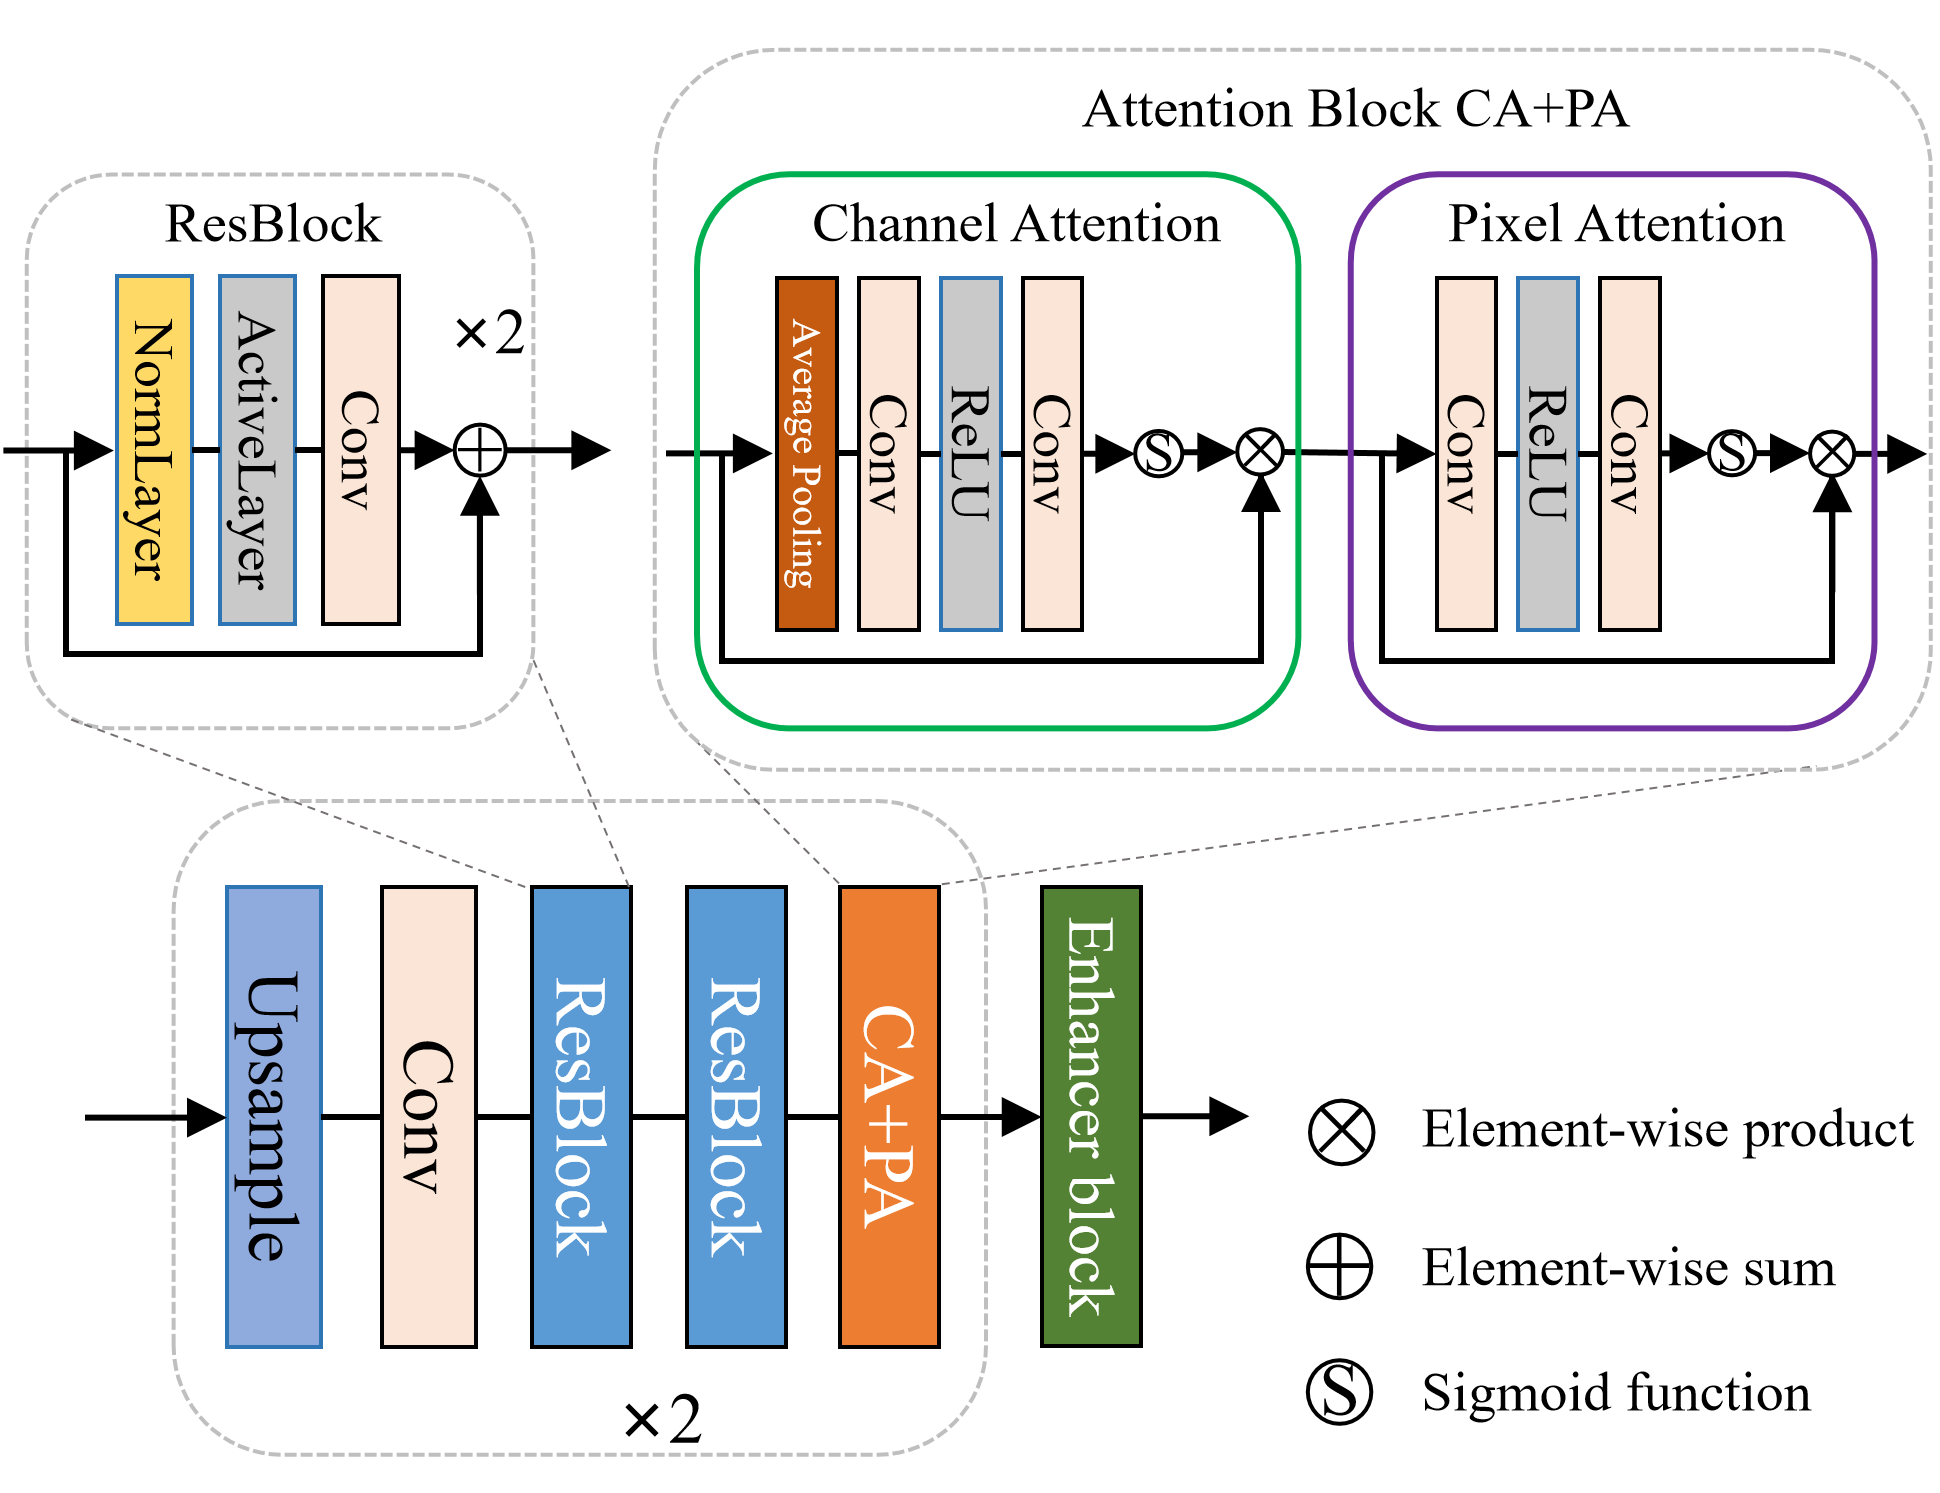
\includegraphics[width=3.5in]{enhanced_decoder}
	\caption{Architecture of our Additional Enhanced Decoder(AED), which consists of upsampling layers, convolutions, residual blocks, channel attention and pixel attention blocks, as well as an enhancer block. }
	\label{fig3}
\end{figure}
\begin{figure}[!t]
	\centering
	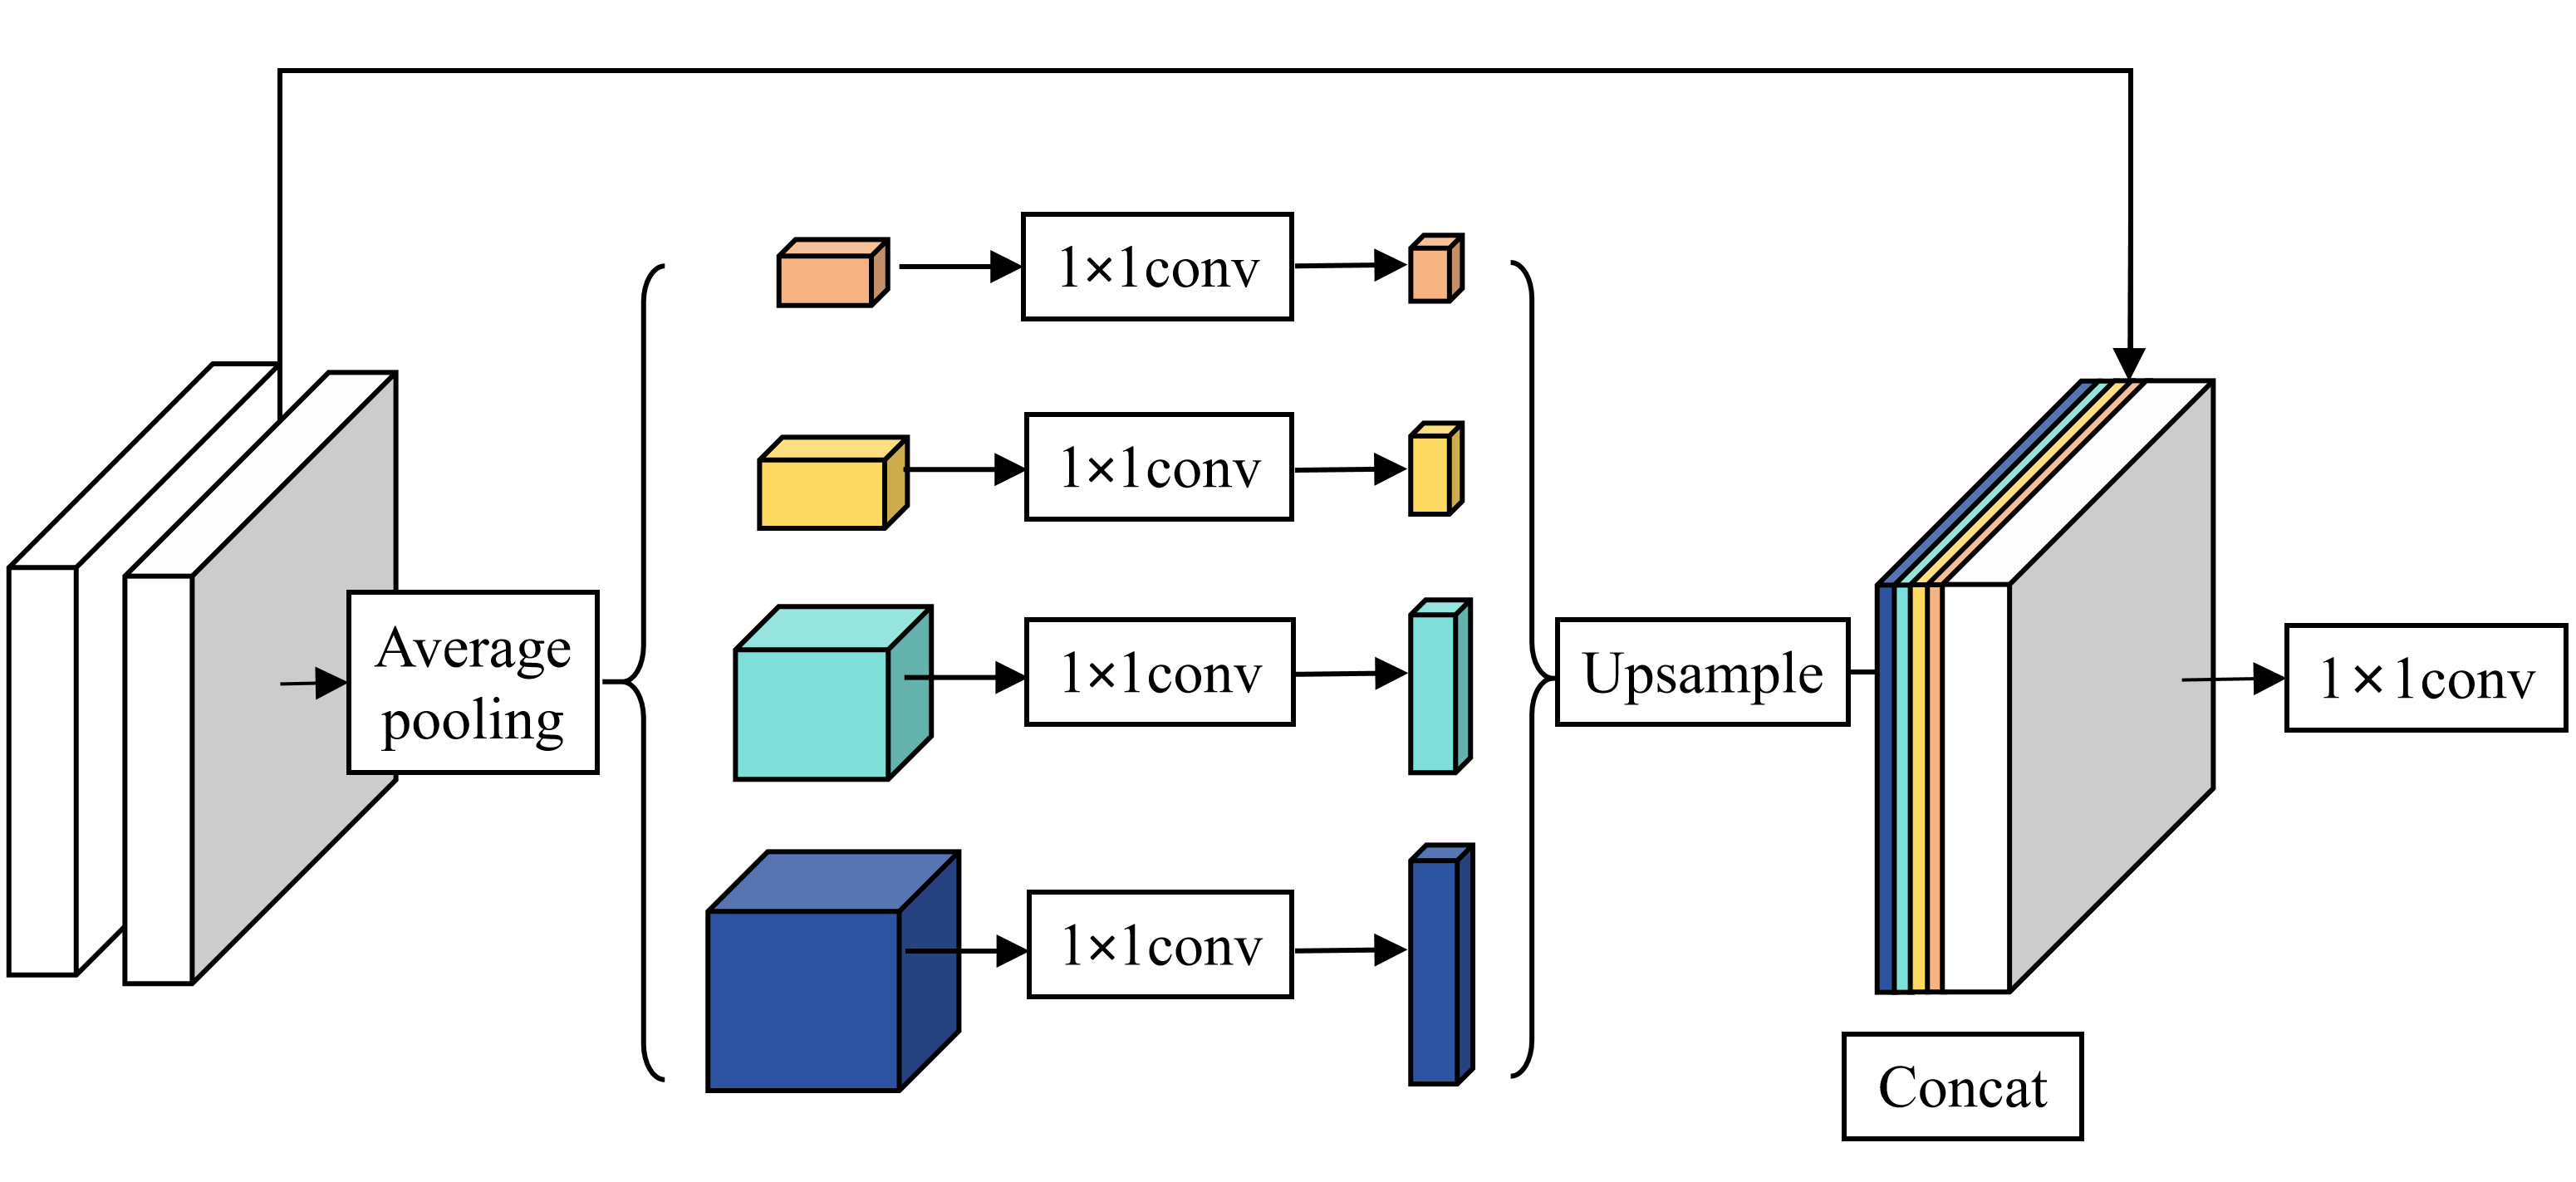
\includegraphics[width=3.5in]{enhancer_block}
	\caption{Detail network structure of the Enhancer Block.}
	\label{fig4}
\end{figure}

{\bf{Dual-branch network structure:}}
In addressing the issue of poor feature extraction in dense hazy regions, we proposes to employ a channel attention branch, using multiple residual and channel convolutions to focus on the dense haze areas to achieve differentiated dehazing effects.
Attention mechanisms enable the network to flexibly focus on the characteristics of the haze, reconstructing high-quality haze-free images. Non-homogeneous and dense haze significantly increases the brightness of its occluded areas. Paying more attention to the restoration of areas with significant brightness variations, such as the sky and snowfields, can avoid over-enhancement issues, thus improving the overall reconstruction performance of the image.

\subsection{High-quality Codebook}
We are inspired by the latest research technology in image generation neighborhoods, VQGAN~\cite{esser2021taming}. While extracting features, we use the pre-trained VQGAN to add image generation capabilities to the dehazing network, thereby helping to restore the image structure and details in heavy haze areas. The overall training is divided into two stages. The first stage requires training the VQGAN network on a high-quality clear dataset to achieve the restoration of image detail textures. In this stage, the network consists of a VQ encoder, codebook, and VQ decoder. The training goal is to obtain a codebook that stores high-quality clear image features and its corresponding VQ decoder. The VQ encoder and decoder adopt a network architecture based on UNet~\cite{ronneberger2015u}. UNet first half is feature extraction, and the second half is upsampling. UNet has been proven to perform well in fields such as image classification and segmentation. Since the encoder's downsampling and feature refinement will lose some edge features, multiple residual structures are used. Through feature concatenation, the retrieval of edge features is achieved, discretization operation is shown in Fig.~\ref{fig2}.

\begin{figure}[!t]
	\centering
	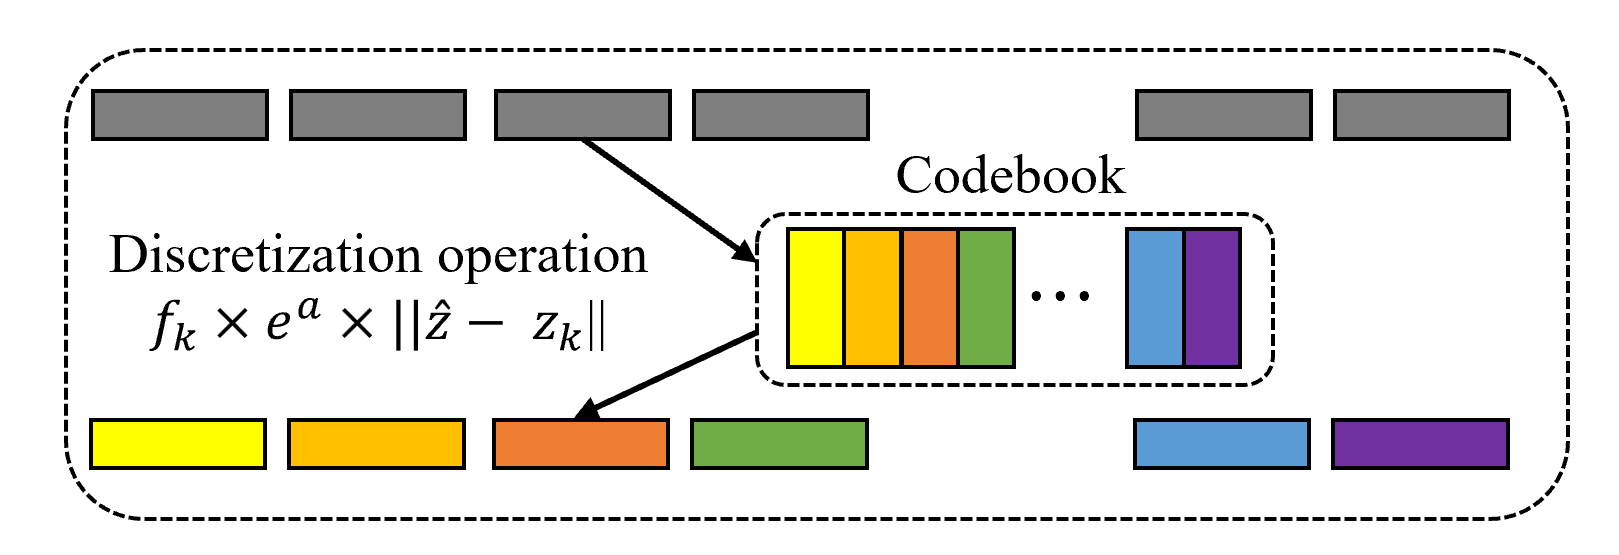
\includegraphics[width=3.5in]{discretization_operation}
	\caption{The discretization operation of the codebook is shown in the figure. The feature map output by the encoder is discretized to form discrete encoded values, represented by gray rectangles. Each discrete encoded value corresponds to an embedding, and all embeddings are stored in an embedding space, which is the codebook. Using the nearest neighbor algorithm to obtain the true embedding in the codebook, represented as a colored rectangular prism, as input to the decoder.}
	\label{fig2}
\end{figure}

Given a high-quality image $x$ as the input to the VQ encoder, an underlying feature map $z$ is output. Then each pixel $z_{ij}$ in $Z$ is matched to the nearest element in the codebook, thereby obtaining the codebook discrete feature map $z^{q}_{ij}$. Subsequently, the discretized features are input into the decoder to obtain the processed image. The entire process can be represented as follows:

\begin{equation}
\label{vq_equation_1}
z_{ij} = E_{vq}(x_{ij})
\end{equation}

\begin{equation}
\label{vq_equation_2}
z_{ij}^{q} = M(\widehat{z}_{ij}) = arg \min_{z_{k} \in Z} (|| \widehat{z}_{ij} - z_{k} ||_{2})
\end{equation}

\begin{equation}
\label{vq_equation_3}
y_{ij} = D_{vq}(z_{ij}^{q})
\end{equation}

The features of a clear image are compressed into short vectors through discretization and stored in a codebook. The discrete codebook compresses the detailed texture features of the image, playing a crucial role in image reconstruction.

During the process of reconstructing an image using a high-quality codebook, the discrete encodings output by the encoder may have difficulty matching the high-quality codebook obtained through training on high-quality clear images due to the presence of haze. Therefore, we need to design a matching operation that utilizes a controllable distance recalculation method to reduce the problem of inconsistent data distribution caused by the domain gap between hazy and non-hazy images, thereby achieving a better reconstruction effect.

Specifically, this involves calculating the distances between the discrete encodings of the hazy image and each encoding in the codebook to find the true encoding with the smallest distance. Then, a weight function $F$ is applied to adjust the final calculated distance, resulting in a matching formula that is expressed as follows:

\begin{equation}
	\label{codebook_matching_equation_2}
	M(z) = arg \min_{z_{k} \in Z} (F(f_{k}, \alpha) \times || \widehat{z} - z_{k} ||)
\end{equation}

\noindent where $f_{k}$ represents the frequency difference between the activation of the hazy image and the clear image on the codebook. The parameter $ \alpha $ is used to adjust the degree of dehazing. $z$ denotes the discretized features of the hazy image, while $z_{k}$ represents the codebook encoding. The notation $||*||$ indicates the distance between the discretized features of the hazy image and the codebook encoding. The expression $arg \min(*)$ means to find the minimum value of the distance.


To facilitate the adjustment of matching results through the parameter $\alpha$ for achieving better defogging effects, we design a weight function as $F(f_{k}, \alpha) = f_{k} \times e^{\alpha} $. Subsequently, we modify the computation method of the activation frequency difference $f_{k}$ in the codebook from statistical analysis to an iterative approach using network learning to obtain optimal values.

\begin{equation}
	\label{codebook_matching_equation_1}
	M(z) = arg \min_{z_{k} \in Z} (f_{k} \times e^{a} \times || \widehat{z} - z_{k} ||)
\end{equation}

Regarding the solution for the parameter $\alpha$, we assume the probability distribution of codebook activations for clear images as $P_{c}$, and the corresponding probability distribution for hazy images as $P_{h}$. The domain gap between the domains of clear and hazy images is transformed into the problem of finding the optimal parameter $\alpha$ in $F(f_{k}, \alpha)$ that minimizes the KL divergence between the probability distributions $P_{c}(x) = z_{k}$ and $P_{h}(x = z_{k} | \alpha) $.


The $KL$ divergence measures the difference between two probability distributions and is commonly used in machine learning to assess the similarity of distributions. In our context, minimizing the $KL$ divergence between $P_{c}$ and $P_{h}$ ensures that the codebook activations for clear and hazy images are as similar as possible, thereby reducing the domain gap and improving the accuracy of the matching process.

To solve for the optimal $\alpha$, we can employ optimization techniques such as gradient descent or other numerical methods. The objective function to be minimized would be the KL divergence between $P_{c}(x) = z_{k}$ and $P_{h}(x = z_{k} | \alpha) $ weighted by  the function $F(f_{k}, \alpha)$.

By iteratively updating $\alpha$ based on the gradients of the objective function, we can find the optimal value that minimizes the $KL$ divergence, thereby improving the matching accuracy and ultimately enhancing the defogging effect.

It is worth noting that the computation of $f_{k}$ and the optimization of $\alpha$ can be integrated into the overall training process of the network. By jointly optimizing the network parameters and the matching criteria, we can achieve better generalization and adaptability to various hazy scenes, leading to more robust and effective dehazing results.

\subsection{Pyramid Neighborhood Attention Encoder}
The VQ encoder performs well when encoding clear images, but it proves insufficient when encoding images with dense haze or non-homogeneous haze. This is primarily because, in the task of dehazing, the encoder must not only extract the general structural texture features from the image but also distinguish the hazy areas within the image. Network architecture of the VQ encoder is relatively shallow, which does not allow it to adequately accomplish this task. In order to fully extract global features such as the texture and structure of hazy images, we designed an encoder based on Pyramid Neighborhood Attention in the prior matching branch. The Pyramid Neighborhood Attention is a variant of the self-attention mechanism found in the Vision Transformer~\cite{dosovitskiy2020image}, serving as an effective and scalable visual sliding window attention mechanism. Neighborhood Attention (NA)~\cite{hassani2023neighborhood, hassani2022dilated} is a per-pixel operation that directs the self-attention (SA)~\cite{vaswani2017attention} towards the nearest neighboring pixels, thus, compared to the quadratic complexity of self-attention, neighborhood attention has linear time and space complexity. Moreover, it surpasses the Vision Transformer and Swin Transformer~\cite{liu2021swin} in downstream visual performance. In our designed Pyramid Neighborhood Attention encoder, four feature maps of different resolution sizes are obtained through the serialization process and two down-sampling operations. By utilizing a pyramid structure and cascading operations, the feature information from each previous layer serves as the input for the next layer, aggregating features from different levels and achieving feature reuse across different scales.

The NA operation can be expressed as:

\begin{equation}
	\label{NA_operation}
	NA_{k} = softmax (\frac{A_{k}}{\sqrt{d}}) V_{k}
\end{equation}

where $A_{k}$ is the attention weight of the input with a neighborhood size of $k$, which is the dot product of the input query projection and its $k$ nearest neighbor key projections. The neighboring value $V_k$ is a matrix whose rows are projections of the $k$ nearest neighboring values of the input, and $\sqrt{d}$ is the scaling parameter.


\subsection{Loss Function}

\begin{figure*}[!t]
	\centering
	\includegraphics[width=7in]{O-HAZE-compare}
	\caption{Visual examples in dataset O-HAZE. From left to right are hazy images, advanced methods for comparison and our method result, and Ground Truth.}
	\label{fig6}
\end{figure*}

\begin{figure*}[!t]
	\centering
	\includegraphics[width=7in]{DENSE-HAZE-compare}
	\caption{Visual examples in dataset DENSE-HAZE. From left to right are hazy images, advanced methods for comparison and our method result, and Ground Truth.}
	\label{fig7}
\end{figure*}

\begin{figure*}[!t]
	\centering
	\includegraphics[width=7in]{NH-HAZE-20-compare}
	\caption{Visual examples in dataset NH-HAZE-20. From left to right are hazy images, advanced methods for comparison and our method result, and Ground Truth.}
	\label{fig8}
\end{figure*}

\begin{figure*}[!t]
	\centering
	\includegraphics[width=7in]{NH-HAZE-21-compare}
	\caption{Visual examples in dataset NH-HAZE-21. From left to right are hazy images, advanced methods for comparison and our method result, and Ground Truth.}
	\label{fig9}
\end{figure*}

\begin{figure*}[!t]
	\centering
	\includegraphics[width=7in]{NH-HAZE-23-compare}
	\caption{Visual examples in dataset NH-HAZE-23. From left to right are hazy images, advanced methods for comparison and our method result, and Ground Truth.}
	\label{fig10}
\end{figure*}

The network training proposed in this paper is divided into two stages in total. The training objective of the first stage is to make the reconstructed image as similar as possible to the original image. During training, the encoder maps the input intermediate features to a network embedding layer called the discrete codebook through discretization. The output of the encoder needs to satisfy the data distribution of the discrete codebook, and the decoder decodes the features that conform to the data distribution of the discrete codebook back into images. The training objective of the second stage is to dehaze. Firstly, the parameters of the following network layers obtained from the first stage are fixed: 

\begin{list}{}{}
	\item{1. High Quality Codebook.}
	
	\item{2. VQ Decoder.}

\end{list}

Then, the remaining parts of the network are trained. Therefore, different loss functions are adopted for different stages of network training in this paper.

{\bf{Stage 1: High Quality Codebook Training.}} For the initial stage of discrete codebook training, the total training loss $L_{vq}$ is divided into the image reconstruction loss $L_{rec}$ and the codebook loss $L_{codebook}$, the loss is defined as

\begin{equation}
\label{vq_loss}
L_{vq} = L_{rec} + L_{codebook}
\end{equation}

The image reconstruction loss can be further divided into the following formulas, where $\hat{x}$ is the output image and $x$ is the input image. $|| * ||_{1}$ represents the $L_{1}$ loss, $L_{per}$ is the perceptual loss, and $L_{adv}$ is the adversarial loss

\begin{equation}
\label{reconstruction_loss}
L_{rec} = || \hat{x} - x ||_{1} + L_{per} + L_{adv}
\end{equation}

Perceptual loss measures the perceptual similarity across the entire feature space. The function denotes the feature maps of the 3rd, 5th, and 8th convolutional layers in the pre-trained VGG16~\cite{simonyan2014very} network (i.e., j=3,5,8). The purpose of using this function is to capture perceptual and semantic information within the images. Perceptual loss is defined as~\cite{johnson2016perceptual}:

\begin{equation}
\label{perceptual_loss}
L_ {perc} = \frac{1}{N} \sum_{j} \frac{1}{C_{j}H_{j}W_{j}} || \phi_(f_{\theta}(x)) - \phi_{j}(y)||_{2}^{2}
\end{equation}

Since pixel-based loss functions cannot provide sufficient supervision on small datasets, an adversarial loss is added to mitigate the shortcomings of the above losses~\cite{zhu2017unpaired}. 

\begin{equation}
\label{adversarial_loss}
L_{adv} = \sum_{n=1}^{N} - \log_{D} (f_{\theta}(x))
\end{equation}

\noindent where D represents the discriminator used during the training of the codebook. N indicates the number of sample data.


The codebook loss can be further divided into the following formula~\cite{chen2022real}:

\begin{equation}
\label{codebook_loss}
\begin{split}
	L_ {codebook} = || sg(\widehat{z}) - z^ {q} ||_{2}^{2} + \beta ||sg(z^{q})- \widehat{z}||_{2}^{2} \\
	+ \gamma ||CONV(z^{q}) - \phi(x)||_{2}^{2}
\end{split}
\end{equation}

\noindent where $sg[*]$ denotes stop-gradient, with $\beta = 0.25$, $\gamma = 0.1$. The last term is a semantically guided regularization item, where $CONV$ signifies a simple convolutional layer and $\phi$ is a pre-trained VGG19~\cite{simonyan2014very}. This loss function primarily measures the quantization error between the output $z$ of the encoder and the discrete vector $z_{q}$.

{\bf{Stage 2: Dehaze Training.}} 

For the second stage of the dehazing task training. Assuming the hazy image input is denoted as $x_h$, and the fog-free ground truth image input as $x_{gt}$, with the dehazing network encoder represented by $E$, the training codebook's encoder by $E_{vq}$, and the training codebook's decoder by $G_{vq}$, and the enhancement decoder by $G$. We can obtain the intermediate features of the hazy image after processing by the encoder $E$, and the intermediate features of the haze-free image after processing by the encoder $E_{vq}$. To control the style difference between the generated images and the fog-free images during the image generation process, we use $\Psi(\cdot)$, which is the Gram matrix, to measure the style loss~\cite{gondal2019unreasonable}. A discriminator $D$ is used to determine whether the generated features are realistic.

Therefore, the loss function for the dehazing stage can be written in the following form:

\begin{equation}
\label{encoder_loss}
\begin{split}
L_{E} =||\widehat{z}_{h} - z^{q}_{t} ||_{2}^{2} + \lambda_{style} ||\Psi(\widehat{z}_{h} - \Psi(z^{q}_{gt}) ||_{2}^{2} \\ 
+ \lambda_{adv}\sum_{i} -E[D(\widehat{z}_{h})]
\end{split}
\end{equation}

The loss function for the remaining part of the network is as follows, where $y$ represents the final output and $\phi$ denotes the pre-trained VGG16~\cite{simonyan2014very}. The gradient of this decoder will not be backpropagated into the encoder.

\begin{equation}
	\label{rest_loss}
	\begin{split}
		L_{remain} =||y - x_{gt} ||_{1} + \lambda_{per} ||\phi(y) - \phi(x_{gt}) ||_{2}^{2}
	\end{split}
\end{equation}



\section{EXPERIMENTS}

 \begin{table*}
	\begin{center}
		\caption{Quantitative Comparison Results of Various Dehazing Methods and Proposed Method on I-HAZE, O-HAZE, DENSE-HAZE, NH-HAZE-20, NH-HAZE-21 and NH-HAZE-23. \textbf{Bold} Indicates the Best and \underline{Underline} Indicates the Second Best.}
		\label{table_compare_with_benchmarks}
		\resizebox*{\linewidth}{!}{
			\begin{tabular}{ c | c | c | c | c | c | c | c | c | c | c | c }
				\hline
				
				\multirow{2}{*}{Dataset} & \multirow{2}{*}{Metric} & DCP\cite{he2010single} & AOD\cite{li2017aod} & GCA\cite{chen2019gated} & FFA\cite{qin2020ffa} & TNN\cite{yu2021two} & DeHamer\cite{guo2022image} & FogRomoval\cite{jin2022structure} & SCA\cite{guo2023scanet} & ConvIR\cite{cui2024revitalizing} & \multirow{2}{*}{ours} \\
				
				& & (TPAMI10) & (ICCV17) & (WACV19) & (AAAI20) & (CVPRW21) & (CVPR22) & (ACCV22) &  (CVPRW23) & (TPAMI24) \\
				\hline

				\multirow{4}{*}{O-HAZE} & PSNR & 12.92 & 17.69 & 19.50 & 22.12 & \textbf{25.54} & 17.02 & 24.61 & 19.47 & \underline{25.25} & 24.54 \\
				& SSIM & 0.50 & 0.62 & 0.66 & 0.77 & 0.78 & 0.43 & 0.75  & 0.74 & \underline{0.78} & \textbf{0.79} \\
				& LIPIS & 0.35 & 0.34 & 0.31 & \underline{0.21} & \textbf{0.20} & 0.29 & 0.28 & 0.39 & 0.33 & 0.24 \\
				\hline
				
				\multirow{4}{*}{DENSE-HAZE} & PSNR & 10.85 & 13.30 & 12.42 & 16.26 & 16.36 & 16.62 & 16.67 & 16.34 & \underline{17.45} & \textbf{17.79} \\
				& SSIM & 0.40 & 0.47 & 0.48 & 0.54 & 0.58 & 0.56 & 0.50 & 0.56 & \textbf{0.64} & \underline{0.62} \\
				& LIPIS & 0.79 & 0.77 & 0.62 & 0.51 & 0.50 & 0.49 & \underline{0.46} & 0.58 & 0.42 & \textbf{0.37} \\
				\hline
				
				\multirow{4}{*}{NH-HAZE-20} & PSNR & 12.29 & 13.44 & 17.58 & 18.51 & 17.18 & 18.53 & \underline{20.99} & 19.52 & 20.65 & \textbf{21.73} \\
				& SSIM & 0.41 & 0.41 & 0.59 & 0.64 & 0.61 & 0.62 & 0.61 & 0.65 & \textbf{0.80} & \underline{0.79} \\
				& LIPIS & 0.56 & 0.54 & 0.31 & 0.26 & 0.28 & 0.26 & 0.23 & 0.55 & \underline{0.20} & \textbf{0.19} \\
				\hline
				
				\multirow{4}{*}{NH-HAZE-21} & PSNR & 11.30 & 13.22 & 18.76 & 20.40 & 20.13 & 18.17 & 18.34 & \underline{21.14} & - & \textbf{21.52} \\
				& SSIM & 0.60 & 0.61 & 0.77 & \underline{0.81} & 0.80 & 0.77 & 0.72 & 0.77 & - & \textbf{0.89} \\
				& LIPIS & 0.50 & 0.49 & 0.24 & \underline{0.15} & \textbf{0.14} & 0.25 & 0.44 & 0.51 & - & 0.20 \\
				\hline
				
				\multirow{4}{*}{NH-HAZE-23} & PSNR & 11.87 & 12.47 & 16.36 & 18.09 & 18.19 & 17.61 & 18.80 & \underline{20.44} & - & \textbf{20.85} \\
				& SSIM & 0.47 & 0.37 & 0.51 & 0.58 & 0.64 & 0.61 & 0.60 & \underline{0.66} & - & \textbf{0.79} \\
				& LIPIS & 0.62 & 0.56 & 0.49 & 0.33 & \underline{0.27} & 0.35 & 0.55 & 0.36 & - & \textbf{0.22} \\
				\hline			
			\end{tabular}
		}
		
	\end{center}
\end{table*}

\subsection{Datasets}
To validate the effectiveness of our proposed model, we conducted experiments on four datasets, namely O-HAZE~\cite{ancuti2018ohaze}, DENSE-HAZE~\cite{ancuti2019dense}, NH-HAZE-20~\cite{ancuti2020ntire}, NH-HAZE-21~\cite{ancuti2021ntire}, and NH-HAZE-23~\cite{ancuti2023ntire}, for the purpose of training and evaluating our model. Specifically, we selected five pairs of images from each dataset for validation and testing, while the remaining images were used for training. More detailed information can be obtained from the accompanying table~\ref{table_dataset}.

The O-HAZE dataset is authentic collection featuring uniform haze conditions, encompassing 45 pairs of outdoor images. These hazy images were captured under genuine atmospheric haze produced by specialized equipment, ensuring their realism and utility for benchmarking dehazing algorithms.

The DENSE-HAZE dataset introduces a novel contribution to the field by focusing on dense, uniform haze scenarios. Comprising 55 pairs of heavily hazy and their corresponding clear images across various outdoor settings, DENSE-HAZE stands out for its portrayal of dense haze conditions recorded through specialized haze-producing machinery. The resultant images are so heavily veiled that the original objects within them are nearly indiscernible, presenting a significant challenge in dehazing tasks compared to conventional datasets. This characteristic makes DENSE-HAZE particularly demanding for testing the robustness and effectiveness of dehazing algorithms under extreme conditions.

The NH-HAZE dataset addresses a critical gap in the field of image dehazing: the scarcity of real-world images with non-uniform haze for reference. Unlike many synthetic datasets, NH-HAZE provides a collection of truly non-homogeneous hazy images paired with their corresponding clear counterparts. The non-homogeneous haze within the NH-HAZE dataset is introduced through the simulation of realistic hazy conditions using professional haze generators, making it a more challenging and practical dataset for evaluating dehazing methods. Its temporal evolution, marked by release dates, allows for further categorization into NH-HAZE-20, NH-HAZE-21, and NH-HAZE-23, containing 40, 25, and 55 image pairs respectively.

\begin{table}
	\begin{center}
		\caption{The details of the datasets used in our experiments}
		\label{table_dataset}
		\begin{tabular}{ c | c | c | c }
			\hline
			Dataset & Train set & Validation set & Image size \\
			\hline
			O-HAZE & 40 & 5 & 2426×2942-5416×3592 \\
			DENSE-HAZE & 50 & 5 & 1600×1200 \\
			NH-HAZE-20 & 50 & 5 & 1600×1200 \\
			NH-HAZE-21 & 20 & 5 & 1600×1200 \\
			NH-HAZE-23 & 35 & 5 & 4000×6000 \\
			\hline			
		\end{tabular}
	\end{center}
\end{table}

\subsection{Implementation Details}
During training, input images were randomly cropped to a size of 256×256 and augmented through scaling, random rotation, and flipping. The Adam optimizer~\cite{kingma2014adam} was employed in this study, with default $\beta_{1}$ and $\beta_{2}$ values set to 0.9 and 0.99, respectively. The initial learning rate was set to 0.0001, and the batch size was set to 1. The model was implemented on an NVIDIA V100 Tensor Core using the Pytorch framework.

\subsection{Evaluation Metrics and Competitors}
Quantitative analysis was conducted using Peak Signal-to-Noise Ratio (PSNR), Structural Similarity index (SSIM)~\cite{wang2004image}, LPIPS~\cite{zhang2018unreasonable} for evaluation. PSNR, measured in decibels (db), represents the ratio of the maximum power of a signal to the noise power that may affect its representation accuracy. A higher PSNR value indicates less distortion in dehazed image. SSIM evaluates image similarity from three aspects: brightness, contrast, and structure, with a value range of $[0,1]$. A higher SSIM value indicates greater similarity between the current image and the Ground Truth. Compared to PSNR, SSIM better aligns with human visual perception in assessing image quality. LPIPS measures the difference between two images by extracting features for each image using deep learning techniques and computing their similarity based on these features.
 
\subsection{Quantitative Evaluations on Benchmarks}
To verify the effectiveness of the network and its generalization ability in difference scenarios, we conduct experiments for comparison. We compare our method with 9 state-of the art dehazing methods, including DCP~\cite{he2010single}, AOD~\cite{li2017aod}, GCA~\cite{chen2019gated}, FFA~\cite{qin2020ffa}, TNN~\cite{yu2021two}, DeHamer~\cite{guo2022image}, FogRemoval~\cite{jin2022structure}, SCA~\cite{guo2023scanet}, ConvIR~\cite{cui2024revitalizing}. The results for the four different quantitative metrics are shown in Table \ref{table_compare_with_benchmarks}.

Fig. \ref{fig6}-\ref{fig10} present the visual comparison between our method and other state-of-the-art algorithms across six dehazing datasets. Visualization of NH-HAZE-21 and NH-HAZE-23 using ITB~\cite{liu2023data} instead of ConvIR. Using NH-HAZE-20 as an example, which is characterized by non-homogeneous haze distribution with certain regions heavily obscured, making background objects barely discernible, our approach effectively mitigates this haze. It produces a color representation and clarity closely aligned with the ground truth, without noticeable chromatic aberrations, achieving a largely dehazed effect. However, in areas with extremely dense haze, the model faces challenges in accurately estimating haze-free conditions, resulting in less precise restoration of textural details in these regions. Despite this, the perceptual effect is significantly improved, with the haze substantially cleared.

In contrast, the DCP algorithm fails to significantly reduce the haze, leaving a pronounced blue cast and severe color distortion throughout the image. While the AOD algorithm avoids obvious color distortions, its dehazing performance is limited in the context of real-world, non-uniform haze scenarios. The GCA method shows some dehazing effect but suffers from severe detail loss in the post-dehazed images, particularly in areas with high haze concentration, where residual white haze remains. Although FFA, TNN, and Dehamer address uneven haze to some extent, they still struggle with detail preservation and color accuracy.

FogRemoval produces superior results in comparison, but ITB processed images exhibit slight color distortions. SCA generally performs well in dehazing but tends to over-smooth regions with fine details, such as densely packed branches, leading to perceptual distortions. In contrast, our method consistently outperforms these alternatives, visually aligning more closely with haze-free images. Most of the haze is effectively removed, and critical textural details are preserved.

\subsection{Ablation Study}
To assess the contribution of each component in our proposed method, we conducted a series of ablation studies. The ablation experiments were conducted on the NH-HAZE-20 dataset, with results summarized in Table~\ref{Ablation_study_1}. And experiments involved the following configurations:

1) Base: Consists of VQ Encoder, VQ Decoder and RSTB~\cite{liang2021swinir}.

2) Base+CB: Includes the codebook(CB).

3) Base+PDiNAT+CB: Replaces RSTB with the proposed PDiNAT.

4) Base+PDiNAT+CB+CAB: Incorporates the channel attention branch(CAB).

5) Base+PDiNAT+CB+CAB+AED: Adds the additional enhancement decoder(AED).

\begin{table}
	\begin{center}
		\caption{Ablation study on the proposed network performance after gradually add modules. The scores are evaluated on NH-HAZE-20 dataset. \textbf{Bold} indicates the best and \underline{underline} indicates the second best.}
		\label{Ablation_study_1}
		\begin{tabular}{c | c | c | c | c }
			\hline
			Index & Method & PSNR & SSIM & LPIPS \\
			\hline
			1 & Base & 18.61 & 0.61 & 0.37 \\
			2 & 1 + CB & 19.41 & 0.62 & 0.31 \\
			3 & 2 + PDiNAT & 20.56 & 0.69 & 0.22 \\
			4 & 3 + CAB & 21.36 & 0.78 & 0.20 \\
			5 & 4 + AED & \textbf{21.73} & \textbf{0.79} & \textbf{0.19} \\
			\hline
		\end{tabular}
	\end{center}
\end{table}

{\bf{Effectiveness of CodeBook.}} The high-quality codebook introduced in this paper effectively compresses the detailed texture features of the image by reconstructing the clear image, encapsulating high-quality prior knowledge. When the codebook is integrated into the Base model, the overall performance improves, with a PSNR increase of 0.8 dB, an SSIM enhancement of 0.01, and an LPIPS reduction of 0.06.

{\bf{Effectiveness of PDiNAT.}} The proposed PDiNAT module enables the model to fully extract local texture and structural features from hazy images. By utilizing a pyramid structure, it aggregates features from different levels, facilitating multi-scale feature reuse. This approach effectively preserves the texture features of hazy images, thereby assisting the subsequent codebook feature matching operation. Experimental results demonstrate that the inclusion of PDiNAT leads to a further performance improvement: PSNR increases by 1.15 dB, SSIM improves by 0.07, and LPIPS decreases by 0.09, compared to the model with the Base configuration.

{\bf{Effectiveness of CAB.}} The CAB module employs a classical channel attention branch commonly used in the dehazing domain, which emphasizes areas with significant brightness variation, such as non-homogeneous fog and dense haze regions. This focus helps mitigate over-enhancement issues and improves the overall image reconstruction performance.

{\bf{Effectiveness of AED.}} The AED module introduces an enhanced decoder based on multiple attention mechanisms, which prioritizes the detailed features of hazy images. This enhancement strengthens the network’s decoding capability, contributing to more accurate and refined reconstruction of hazy scenes.

As observed, the model's performance improves progressively as more components are integrated. Fig. \ref{Ablation_study_2} illustrates the PSNR performance of networks with different modules at various iterations. As shown, the application of the modules proposed in this paper leads to a significant improvement in PSNR, indirectly validating the effectiveness of the proposed components.

\begin{figure}[!t]
	\centering
	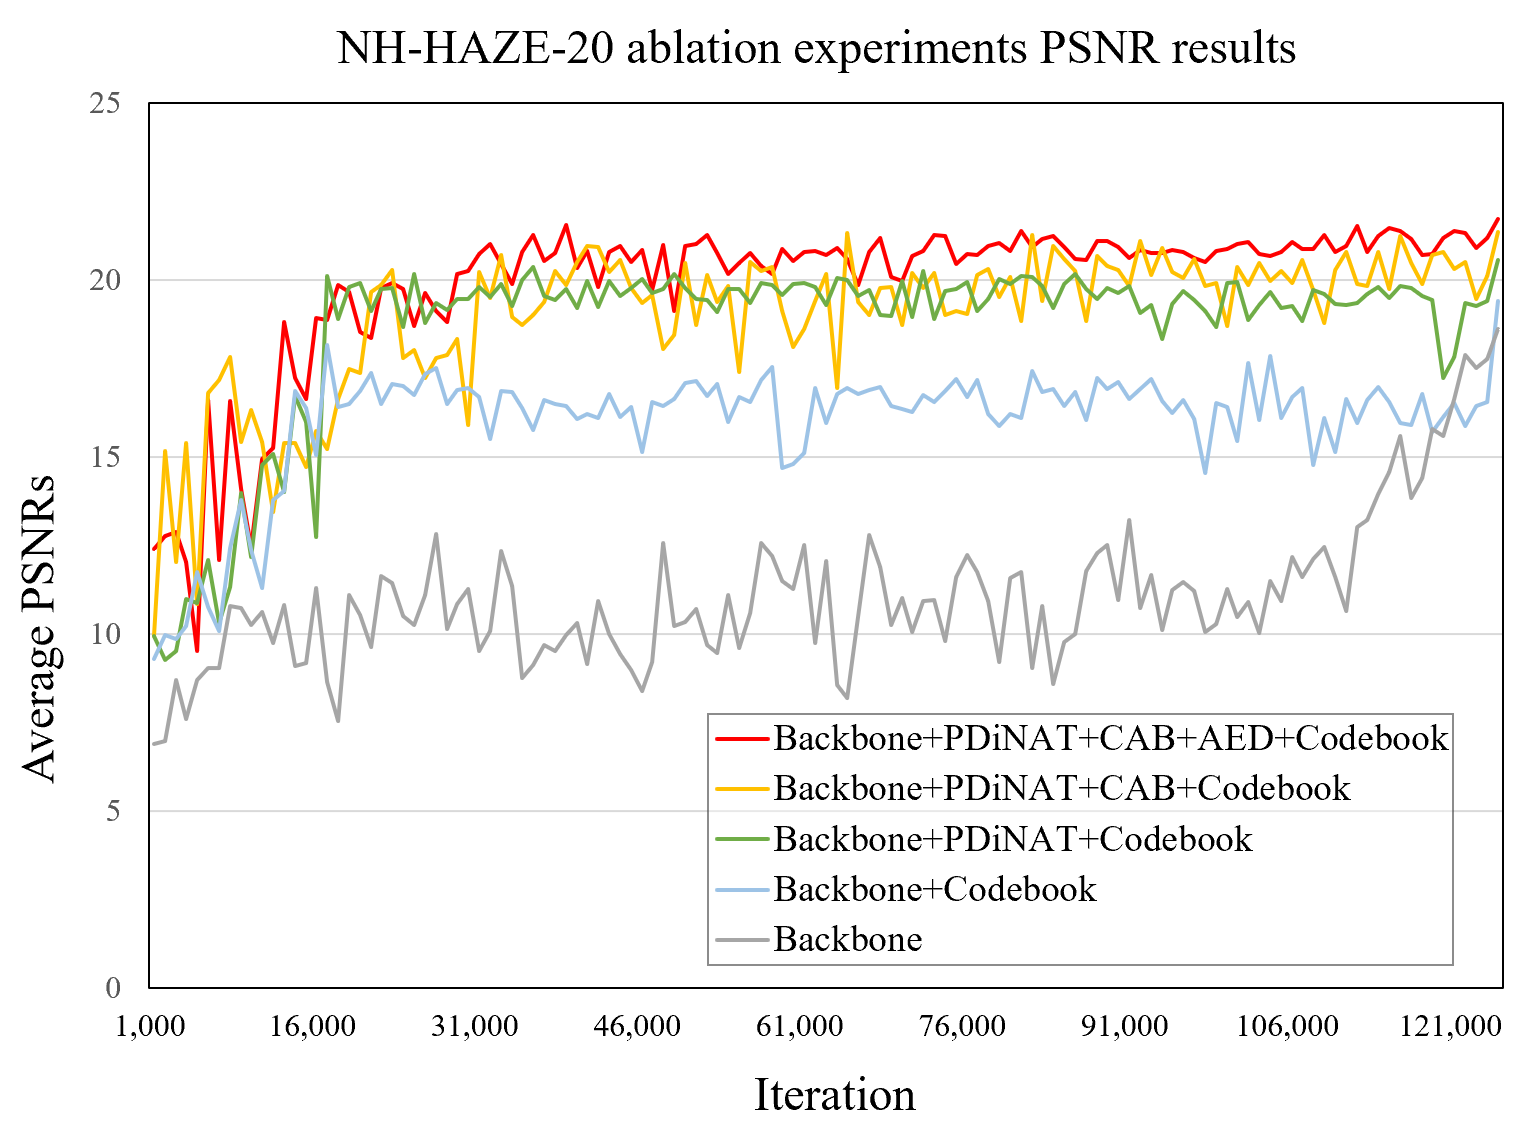
\includegraphics[width=3.5in]{ablation_experiments}
	\caption{The ablation experiments on the NH-HAZE-20 dataset show the PSNR variation curves for different experimental configurations as the number of iterations increases.}
	\label{Ablation_study_2}
\end{figure}


\section{CONCLUSION}
In this paper, we propose a two-branch neural network for non-homogeneous dehazing via high quality codebook and prove its strong power in various dehazing tasks. Subsequently, we proposed a feature pyramid encoder based on dilated neighborhood attention, which can effectively extract features of haze distribution in images through multi-scale feature maps. In order to enhance the decoding capability of the network, we have designed an enhanced decoder that utilizes multiple attention and enhancement blocks to restore the structure and detailed features of the image. Finally, extensive experiments have shown that our method has significant advantages in non-homogeneous datasets.


\bibliographystyle{IEEEtran}
\bibliography{references}{}


\end{document}


